\section{Construction}
The dc-motor needs a housing of some kind and a way of mounting the rotating pcb.
These mounts were chosen to be 3D printed, due to the ease of doing 3D printing, if you have a 3D CAD model.

A housing was drawn in 3D, with the motor in the center, and a hole for a shaft at the side. 
A picture of the housing can be seen in figure \ref{fig:housing3D}.
The motor is then mounted with screws through the small holes in the top.

The rotating pcb is not mounted directly on the shaft of the motor due to the speed of the motor.
Since the motor does 6000 rpm at 100 \% duty cycle, 6V, which is too fast due to greater speeds means greater instability, so gearing has to be 1.
Another great property of gearing the motor, other than increasing the range of the duty cycle.
This gear was mounted on a shaft that was also 3D printed, which was inserted into a bearing, mounted in the big hole in the housing.

\begin{figure}
 \centering
 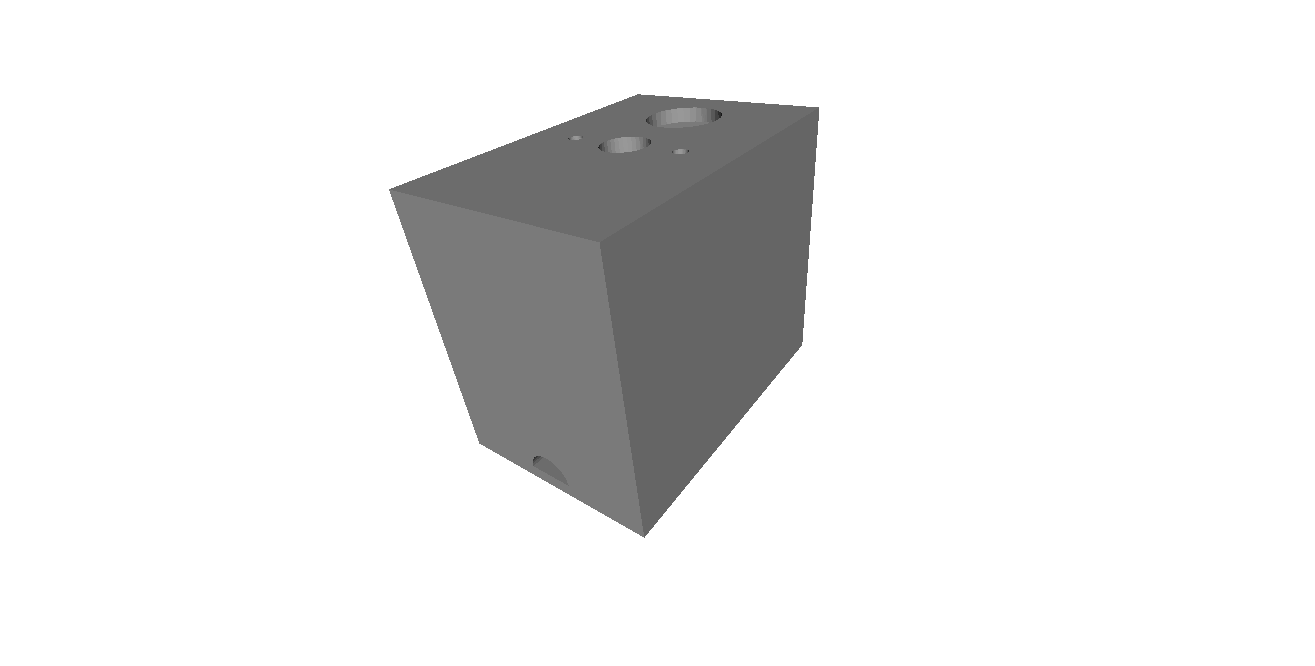
\includegraphics[width=\textwidth]{img/housing3D}
 \caption{Snapshot of the housing 3D drawing}
 \label{fig:housing3D}
\end{figure}

\begin{figure}
 \centering
 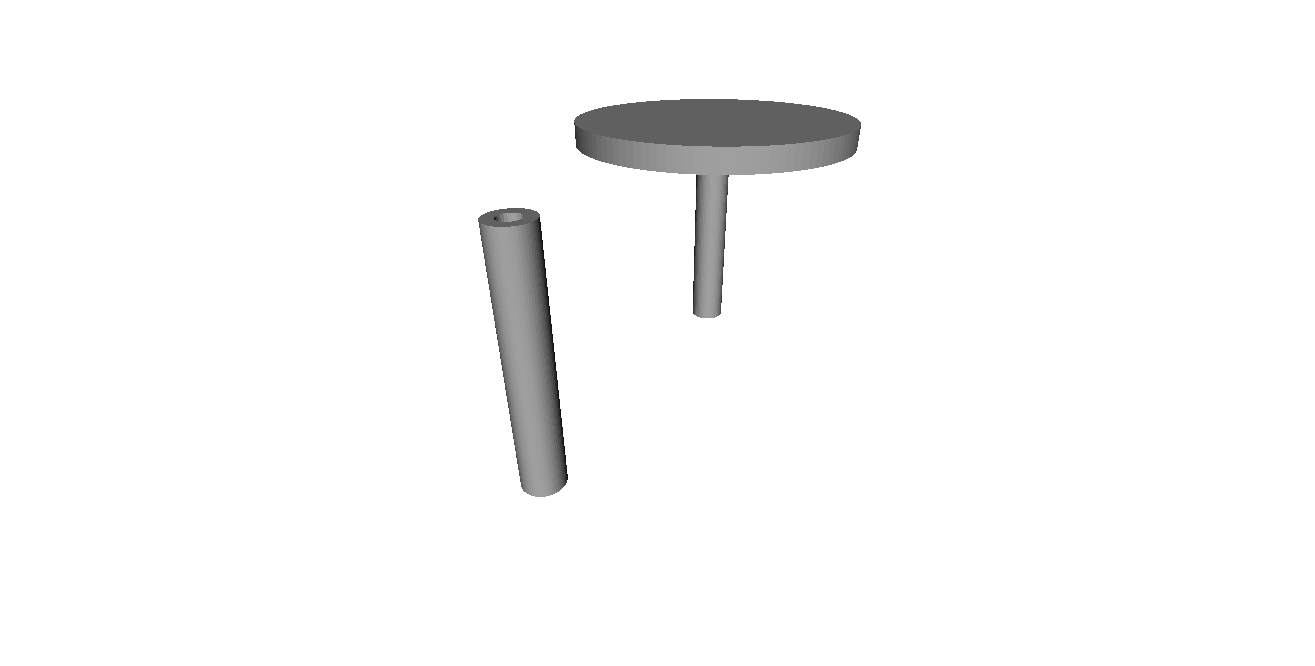
\includegraphics[width=\textwidth]{img/shaft_3d}
 \caption{Snapshot of the shaft 3D drawing}
 \label{fig:shaft3D}
\end{figure}

When running at high speed the most important thing, construction wise, is to make the system as stable as possible to reduce shaking.
One way to do this is to make the board twice the length, so the shaft goes through the center of the board, which should make the weight distribution almost even.